\section{Background}
\subsection{Probabilistic Databases}
Probabilistic Databases arose out of the need to model large amounts of imprecise data.  In the Possible Worlds Data Model \cite{Dalvi07}, let $\mathbf{I}=\{I_{1},I_{2},...,I_{N}\}$ be the set of all possible instances of a typical relational database.  A PDB is the set $(I_{i},p(I_{i}))$ of all instance-probability pairs, where $p(I_{i})\rightarrow[0,1]$ such that $\sum_{i=1}^{N}p(I_{i})=1$.  Queries may be modified to return probabilistic results, though the number of possible worlds may grow exponentially with the size of the database.  It is for this reason that queries generally return only the \textit{top k} most probable results.  A number of implementations of PDBs currently exist, including TRIO \cite{DBLP:conf/vldb/AgrawalBSHNSW06}, MystiQ \cite{Boulos:2005:MSF:1066157.1066277}, MayBMS \cite{Huang09maybms:a}, and Orion \cite{DBLP:conf/comad/SinghMMPHS08}.

\subsection{Probabilistic Graphical Models}
Probabilistic Graphical Models (PGMs) \cite{Koller+Friedman:09, Jordan98} are compact graph structures used to encode the conditional independence properties between random variables.  Bayesian Networks and Markov Networks are structured as directed acyclic graphs and undirected graphs, respectively.  The random variables are represented by nodes in the graph, while dependence relationships are modeled by the edges between them.  PGMs provide structure which aids in the inference and learning associated with probabilistic models.

\begin{figure}
\centering
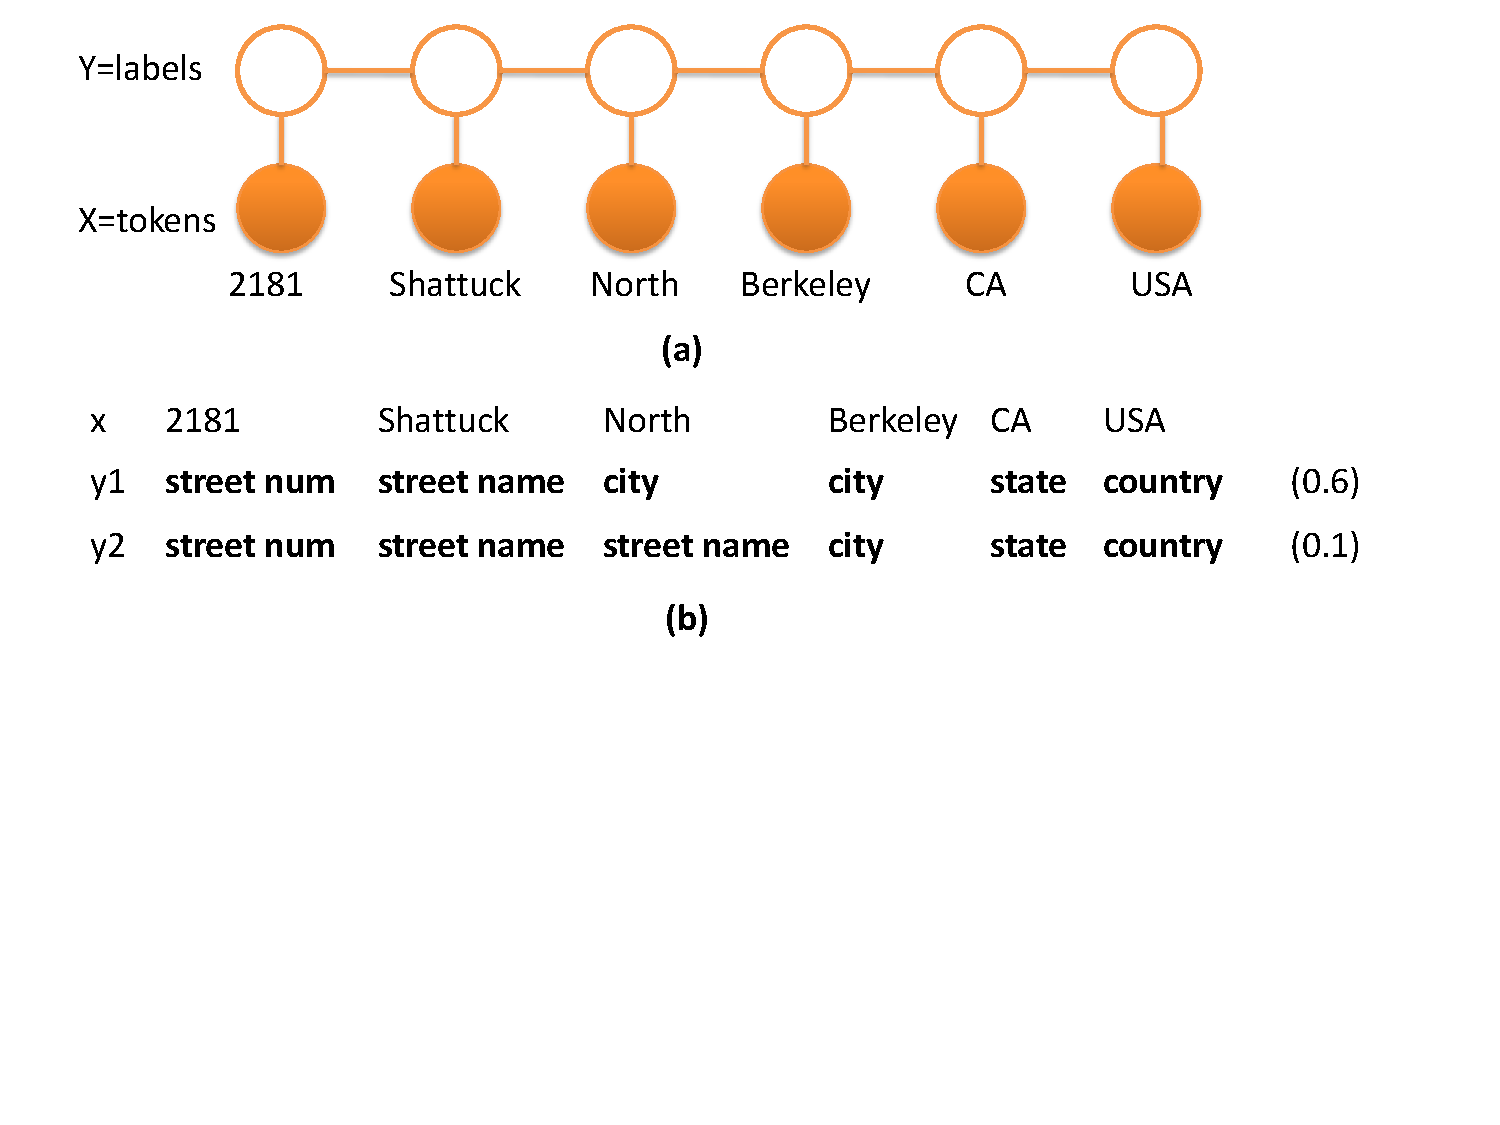
\includegraphics[width=0.52\textwidth]{images/CRF1.pdf}
\caption[example]{\label{fig:CRFexample}(a). Conditional Random Field applied to labeling an address sequence. (b). Possible label sequences along with their associated probabilities.}
\end{figure}

A popular graphical model used extensively in shallow parsing, named entity recognition, and gene finding among others is the Conditional Random Field (CRF) \cite{Lafferty01}.  A CRF is a discriminative undirected PGM pictured in Figure \ref{fig:CRFexample}(a) which is similar to a Hidden Markov Model (HMM), but able to take advantage of a greater set of overlapping features.  Given a set of observed sequence tokens $\mathbf{x}$, such as the words constituting a sentence, a CRF attempts to model the underlying hidden label sequence $\mathbf{y}$ by modeling the conditional distribution
\begin{equation}
\label{eq:CRFeq}
p(\mathbf{y}|\mathbf{x}) = \frac{1}{Z}exp \big{(} \sum_{t=1}^{T}\sum_{k}\lambda_{k}f_{k}(\mathbf{y}_{t},\mathbf{y}_{t-1},\mathbf{x},t)\big{)},
\end{equation}
where $Z$ is a global normalization factor, $T$ is the length of the sequence, and the $\lambda_{k}$ are learned parameters used to weight a set of fixed \textit{features} $f_{k}$. The features are associated with relationships between hidden labels and the observation sequence $\mathbf{x}$.  An example feature in an address labeling task is \textit{"the previous label is a number and the observed sequence is capitalized"}, in which case the value associated with the current label being a street name would be much higher than that for any other label.  The label sequence $\mathbf{y}$ which maximizes equation \ref{eq:CRFeq} can be found by a Viterbi algorithm similar that of a HMM.

\subsection{PGMs in PDBs}
Early probabilistic databases were forced to make simplistic assumptions about the data (such as complete independence among tuples) as well as being confined to a restricted subset of queries expressable in traditional query language.  A number of new systems have attempted to combat this by modeling a PGM directly within the database.  BayesStore \cite{Wang08} explicitly represents uncertainty through the use of Bayesian Networks as first class citizens and PrDB \cite{Sen09} casts query evaluation as inference in a graphical model.

\subsection{Entropy}
The use of entropy as a measure of the uncertainty of a random variable (RV) was first introduced by Shannon \cite{Shannon48} in his seminal paper on information theory.  The entropy, defined for a random variable $X$ with discrete probability mass distribution $p$ is 
\begin{equation}
H(X) = \sum_{i=1}^{n}p(x_{i})log(p(x_{i})),
\end{equation}
where $i$ runs over all possible instances of the random variable.  The entropy measures the spread among the probability of each instance.  A roughly uniform distribution has high entropy and corresponds to a high degree of uncertainty.  The entropy becomes the key metric for question formulation as we discuss later.

\subsection{Amazon Mechanical Turks}
The Amazon Mechanical Turk (AMT) infrastructure is a marketplace for distributed human computation.  Requesters post Human Intelligence Tasks (HITs) such as image annotation and text translation and labeling to be completed by workers drawn from a pool of hundreds of thousands.  Most micro-tasks are trivial for humans, but difficult to do automatically through SML.  The structure of AMT allows for workers to be compensated and produce results much quicker than by traditional means.
